\documentclass[12pt,a4paper]{article}
\usepackage[a4paper,margin=1in]{geometry}
\usepackage{times}
\usepackage{setspace}
\usepackage{graphicx}
\usepackage{float}
\usepackage{booktabs}
\usepackage{array}
\usepackage{tabularx}
\usepackage{amsmath,amssymb}
\usepackage{xcolor}
\usepackage{listings}
\usepackage{fancyvrb}
\usepackage{tikz}
\usepackage{hyperref}
\usepackage{enumitem}
\usepackage{fancyhdr}
\usepackage{titlesec}
\usetikzlibrary{shapes.geometric,arrows.meta,positioning}
\hypersetup{colorlinks=true,linkcolor=blue,citecolor=blue,urlcolor=blue,
pdftitle={ML-Assisted Intelligent Compiler for Automated Syntax Error Detection and Recovery}}
\onehalfspacing
\setlength{\headheight}{15pt}
\pagestyle{fancy}
\fancyhf{}
\fancyhead[L]{Compiler Design Lab -- CSE3024}
\fancyhead[R]{VIT-AP University}
\fancyfoot[C]{\thepage}
\definecolor{codegreen}{rgb}{0,0.5,0}
\definecolor{codegray}{rgb}{0.5,0.5,0.5}
\definecolor{codepurple}{rgb}{0.58,0,0.82}
\lstset{basicstyle=\ttfamily\scriptsize,keywordstyle=\color{blue},
commentstyle=\color{codegreen},stringstyle=\color{codepurple},
numbers=left,numberstyle=\tiny\color{codegray},stepnumber=1,numbersep=6pt,
frame=single,breaklines=true,showstringspaces=false,columns=fullflexible}
\titleformat{\section}{\large\bfseries}{\thesection.}{0.5em}{}
\titleformat{\subsection}{\normalsize\bfseries}{\thesubsection}{0.5em}{}
\begin{document}
\begin{titlepage}
\begin{center}
\vspace*{0.5cm}
{\Large\bfseries VIT-AP UNIVERSITY}\\[0.3cm]
{\large Amaravati, Andhra Pradesh, India}\\[1.0cm]
{\Large\bfseries COMPILER DESIGN LAB REPORT}\\[0.4cm]
{\large \textbf{Subject Name: Compiler Design Lab}}\\[0.15cm]
{\large \textbf{Course Code: CSE3024}}\\[1cm]
{\LARGE\bfseries ML-Assisted Intelligent Compiler for\\
Automated Syntax Error Detection and Recovery}\\[1.2cm]
\textbf{Submitted by}\\[0.4cm]
\begin{tabular}{ll}
\textbf{Student 1} & \textbf{Regd. No.:} 24BCB7033\\[0.4cm]
\textbf{Student 2} & \textbf{Regd. No.:} 24BCB7177
\end{tabular}\\[1.2cm]
\textbf{Under the Guidance of}\\[0.3cm]
\textbf{Dr. Prakash Kumar Sarangi}\\[1cm]
{\large School of Computer Science and Engineering (SCOPE)\\
VIT-AP University\\Amaravati, Andhra Pradesh, India}\\[0.4cm]
{\large Academic Year 2026--2027}
\end{center}
\end{titlepage}

\section*{Abstract}
Compiler errors can be difficult for beginner programmers to understand and fix. This project presents an educational prototype of an ML-assisted intelligent compiler that detects lexical and syntax errors, classifies them, provides correction suggestions, and attempts to continue parsing after an error. The prototype includes a tokenizer, a recursive-descent parser for a small C-like language, structured diagnostics, and panic-mode error recovery. An optional TF--IDF and Logistic Regression classifier demonstrates how machine-learning methods can be included in error categorization. Rule-based parser diagnostics remain authoritative so that the recovery behavior is predictable. The project reports tokens, an abstract syntax tree (AST), error messages, suggested fixes, and test results. Four unit tests cover valid input, missing semicolons, lexical errors, and parser recovery. This is a learning prototype rather than a full C compiler; its supported grammar and ML component are deliberately limited.
\textbf{Keywords:} Compiler Design, Lexical Analysis, Syntax Analysis, Error Classification, Error Recovery, Machine Learning.

\newpage
\section{Introduction}
A compiler translates source code into a representation that can be executed or further processed. Lexical analysis converts characters into tokens, while syntax analysis checks whether those tokens follow the grammar. When code is incorrect, a compiler should report a useful location and explanation. Error recovery is also important because stopping at the first error prevents a learner from discovering other problems in the same program.

\subsection{Problem Statement}
Traditional beginner-level compiler exercises often identify a syntax error but provide limited explanation or recovery. The problem addressed in this project is how to combine rule-based parsing with a lightweight ML demonstration to classify errors, suggest fixes, and resume analysis after common mistakes.

\subsection{Objectives}
\begin{enumerate}
\item Tokenize source text and identify unexpected characters.
\item Parse a small C-like language using recursive-descent methods.
\item Detect and classify common syntax errors.
\item Provide human-readable suggestions and simple recovery actions.
\item Demonstrate an optional TF--IDF and Logistic Regression classifier.
\item Test the implementation and include actual program output in this report.
\end{enumerate}

\subsection{Scope}
The supported subset includes variable declarations, assignments, \texttt{print(...);}, \texttt{return}, identifiers, numbers, addition, subtraction, and parentheses. It is not intended to compile full C or C++ programs. Multiplication and division tokens are recognized lexically but are not fully implemented as expression operators in the parser.

\section{Related Work}
Classical compiler design separates analysis from synthesis. Lexical analyzers identify tokens, parsers construct syntactic structure, semantic analysis checks contextual rules, and later stages generate or optimize code. Error-recovery techniques such as panic-mode recovery skip input until a synchronization token is found. Machine-learning text classifiers can be used to rank or categorize diagnostic messages, but they require representative training examples and careful evaluation.

\begin{table}[H]
\centering
\caption{Techniques used in the prototype}
\begin{tabularx}{\textwidth}{p{3cm}X}
\toprule
\textbf{Technique} & \textbf{Purpose}\\\midrule
Regular-expression lexer & Converts source characters into tokens and flags unknown characters.\\
Recursive-descent parser & Checks statement and expression structure.\\
Rule-based diagnostics & Produces location, error category, explanation, and correction hint.\\
Panic-mode recovery & Skips to a semicolon or end of input to continue parsing.\\
TF--IDF + Logistic Regression & Optional illustrative text-classification component.\\
\bottomrule
\end{tabularx}
\end{table}

\section{Proposed Methodology}
The system follows a small compiler pipeline: source input, lexical analysis, syntax analysis, diagnostic generation, recovery, and report generation. A compact ML classifier is trained on synthetic diagnostic examples at runtime when scikit-learn is available. If it is unavailable, the program still runs using rule-based classifications.

\subsection{System Workflow}
\begin{figure}[H]
\centering
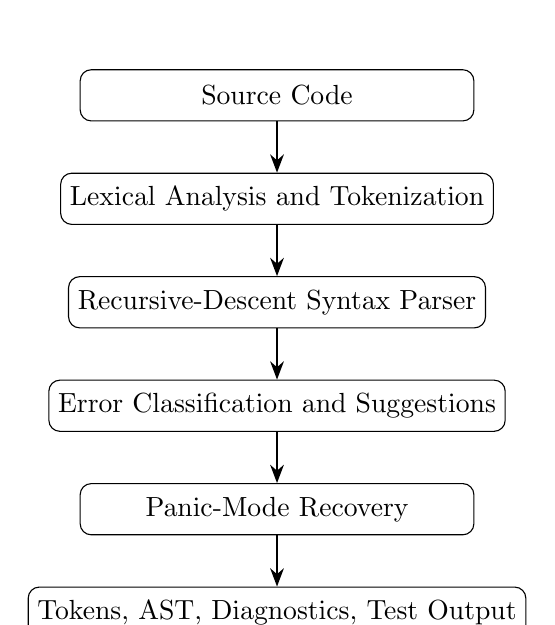
\begin{tikzpicture}[node distance=0.65cm,box/.style={rectangle,rounded corners,draw,minimum width=5.0cm,minimum height=0.65cm,align=center},arrow/.style={-{Stealth},thick}]
\node[box] (src) {Source Code};
\node[box,below=of src] (lex) {Lexical Analysis and Tokenization};
\node[box,below=of lex] (parse) {Recursive-Descent Syntax Parser};
\node[box,below=of parse] (diag) {Error Classification and Suggestions};
\node[box,below=of diag] (rec) {Panic-Mode Recovery};
\node[box,below=of rec] (out) {Tokens, AST, Diagnostics, Test Output};
\draw[arrow] (src)--(lex);\draw[arrow] (lex)--(parse);\draw[arrow] (parse)--(diag);\draw[arrow] (diag)--(rec);\draw[arrow] (rec)--(out);
\end{tikzpicture}
\caption{Workflow of the proposed intelligent compiler prototype.}
\end{figure}

\subsection{Lexical Analysis}
The lexer scans the input and recognizes numbers, identifiers, keywords, operators, parentheses, commas, and semicolons. Whitespace is ignored while line and column positions are tracked. Any unrecognized character generates a lexical diagnostic.

\subsection{Syntax Analysis}
The parser processes declarations, assignments, print statements, and return statements. Expressions are represented as nested dictionary nodes similar to a simplified AST. For example, \texttt{x = a + b;} contains an assignment node with a binary-expression child.

\subsection{Error Classification and Recovery}
Each diagnostic stores its line, column, category, message, suggestion, and recovery action. When a semicolon is missing, the parser reports an insertion suggestion. For unexpected statements, panic-mode recovery advances to a semicolon or end of input, helping the parser continue instead of becoming stuck. The optional ML model is illustrative and trained on a small synthetic set; it should not be considered a validated production classifier.

\subsection{Algorithm}
\begin{enumerate}
\item Read source program.
\item Convert characters into tokens and collect lexical errors.
\item Parse statements and expressions into an AST.
\item Record syntax errors with line and column positions.
\item Generate suggestions and recover at synchronization points.
\item Print tokens, AST statement counts, and diagnostics.
\item Run unit tests to verify representative cases.
\end{enumerate}

\section{Implementation}
The complete implementation is provided in the project ZIP under \texttt{src/compiler.py}. The code below is included in the report for reproducibility.

\subsection{Complete Source Code}
\lstinputlisting[language=Python]{src/compiler.py}

\section{Results and Discussion}
The program was executed on one valid input and three deliberately incorrect inputs. The following output is captured from the included implementation; it is not fabricated performance data.

\subsection{Actual Demonstration Output}
\lstinputlisting[caption={Captured program output}]{outputs/sample_output.txt}

\subsection{Unit Test Results}
Four unit tests were executed: valid program acceptance, missing-semicolon detection, lexical-error detection, and parser recovery. All four tests passed in the recorded run.

\lstinputlisting[caption={Captured unit-test output}]{outputs/test_results.txt}

\subsection{Result Analysis}
The valid program was accepted and tokenized. For malformed input, the system identified a missing semicolon, a missing closing parenthesis, and an unexpected character. It displayed a message and a suggested correction, and continued parsing where possible. A lexical error can cause additional parser errors because the remaining token stream may no longer fit the expected grammar; this behavior is visible in the sample output and is a limitation that could be improved with more sophisticated recovery.

\subsection{Limitations}
\begin{itemize}
\item The grammar covers only a small C-like language subset.
\item Semantic checks such as undeclared variables and type compatibility are not implemented.
\item The ML classifier uses a very small synthetic training set and is only a demonstration.
\item Recovery may produce cascading errors after one invalid token.
\item No claim of execution-speed improvement is made; the project evaluates functional behavior using test cases.
\end{itemize}

\section{Conclusion and Future Work}
This project demonstrates an intelligent compiler prototype that combines tokenization, recursive-descent parsing, syntax-error diagnostics, correction suggestions, and panic-mode recovery. An optional text classifier illustrates a possible role for ML in error categorization, while deterministic parser rules maintain predictable behavior. The recorded unit tests passed for the included cases. Future work can extend the grammar, add semantic analysis, use a larger labeled error dataset, evaluate classification precision and recall, rank multiple correction candidates, and integrate a parser generator or IDE interface.

\section*{References}
\begin{enumerate}[label={[}\arabic*{]}]
\item A. V. Aho, M. S. Lam, R. Sethi, and J. D. Ullman, \textit{Compilers: Principles, Techniques, and Tools}, 2nd ed., Pearson, 2006.
\item K. D. Cooper and L. Torczon, \textit{Engineering a Compiler}, 2nd ed., Morgan Kaufmann, 2011.
\item C. Manning, P. Raghavan, and H. Schütze, \textit{Introduction to Information Retrieval}, Cambridge University Press, 2008.
\item scikit-learn developers, ``Text feature extraction'' and ``Logistic Regression,'' scikit-learn documentation, https://scikit-learn.org/.
\end{enumerate}
\end{document}
